\documentclass[twoside]{book}

% Packages required by doxygen
\usepackage{fixltx2e}
\usepackage{calc}
\usepackage{doxygen}
\usepackage[export]{adjustbox} % also loads graphicx
\usepackage{graphicx}
\usepackage[utf8]{inputenc}
\usepackage{makeidx}
\usepackage{multicol}
\usepackage{multirow}
\PassOptionsToPackage{warn}{textcomp}
\usepackage{textcomp}
\usepackage[nointegrals]{wasysym}
\usepackage[table]{xcolor}

% Font selection
\usepackage[T1]{fontenc}
\usepackage[scaled=.90]{helvet}
\usepackage{courier}
\usepackage{amssymb}
\usepackage{sectsty}
\renewcommand{\familydefault}{\sfdefault}
\allsectionsfont{%
  \fontseries{bc}\selectfont%
  \color{darkgray}%
}
\renewcommand{\DoxyLabelFont}{%
  \fontseries{bc}\selectfont%
  \color{darkgray}%
}
\newcommand{\+}{\discretionary{\mbox{\scriptsize$\hookleftarrow$}}{}{}}

% Page & text layout
\usepackage{geometry}
\geometry{%
  a4paper,%
  top=2.5cm,%
  bottom=2.5cm,%
  left=2.5cm,%
  right=2.5cm%
}
\tolerance=750
\hfuzz=15pt
\hbadness=750
\setlength{\emergencystretch}{15pt}
\setlength{\parindent}{0cm}
\setlength{\parskip}{3ex plus 2ex minus 2ex}
\makeatletter
\renewcommand{\paragraph}{%
  \@startsection{paragraph}{4}{0ex}{-1.0ex}{1.0ex}{%
    \normalfont\normalsize\bfseries\SS@parafont%
  }%
}
\renewcommand{\subparagraph}{%
  \@startsection{subparagraph}{5}{0ex}{-1.0ex}{1.0ex}{%
    \normalfont\normalsize\bfseries\SS@subparafont%
  }%
}
\makeatother

% Headers & footers
\usepackage{fancyhdr}
\pagestyle{fancyplain}
\fancyhead[LE]{\fancyplain{}{\bfseries\thepage}}
\fancyhead[CE]{\fancyplain{}{}}
\fancyhead[RE]{\fancyplain{}{\bfseries\leftmark}}
\fancyhead[LO]{\fancyplain{}{\bfseries\rightmark}}
\fancyhead[CO]{\fancyplain{}{}}
\fancyhead[RO]{\fancyplain{}{\bfseries\thepage}}
\fancyfoot[LE]{\fancyplain{}{}}
\fancyfoot[CE]{\fancyplain{}{}}
\fancyfoot[RE]{\fancyplain{}{\bfseries\scriptsize Generated by Doxygen }}
\fancyfoot[LO]{\fancyplain{}{\bfseries\scriptsize Generated by Doxygen }}
\fancyfoot[CO]{\fancyplain{}{}}
\fancyfoot[RO]{\fancyplain{}{}}
\renewcommand{\footrulewidth}{0.4pt}
\renewcommand{\chaptermark}[1]{%
  \markboth{#1}{}%
}
\renewcommand{\sectionmark}[1]{%
  \markright{\thesection\ #1}%
}

% Indices & bibliography
\usepackage{natbib}
\usepackage[titles]{tocloft}
\setcounter{tocdepth}{3}
\setcounter{secnumdepth}{5}
\makeindex

% Custom commands
\newcommand{\clearemptydoublepage}{%
  \newpage{\pagestyle{empty}\cleardoublepage}%
}

\usepackage{caption}
\captionsetup{labelsep=space,justification=centering,font={bf},singlelinecheck=off,skip=4pt,position=top}

%===== C O N T E N T S =====

\begin{document}

% Titlepage & ToC
\pagenumbering{alph}
\begin{titlepage}
\vspace*{7cm}
\begin{center}%
{\Large R-\/\+Type }\\
\vspace*{1cm}
{\large Generated by Doxygen 1.8.12}\\
\end{center}
\end{titlepage}
\clearemptydoublepage
\pagenumbering{roman}
\tableofcontents
\clearemptydoublepage
\pagenumbering{arabic}

%--- Begin generated contents ---
\chapter{Namespace Index}
\section{Namespace List}
Here is a list of all namespaces with brief descriptions\+:\begin{DoxyCompactList}
\item\contentsline{section}{{\bf compile\+\_\+time} }{\pageref{namespacecompile__time}}{}
\item\contentsline{section}{{\bf ecs} }{\pageref{namespaceecs}}{}
\item\contentsline{section}{{\bf ecs\+::database} }{\pageref{namespaceecs_1_1database}}{}
\item\contentsline{section}{{\bf entity\+\_\+component\+\_\+system} }{\pageref{namespaceentity__component__system}}{}
\item\contentsline{section}{{\bf entity\+\_\+component\+\_\+system\+::component} }{\pageref{namespaceentity__component__system_1_1component}}{}
\item\contentsline{section}{{\bf entity\+\_\+component\+\_\+system\+::database} }{\pageref{namespaceentity__component__system_1_1database}}{}
\item\contentsline{section}{{\bf entity\+\_\+component\+\_\+system\+::entity} }{\pageref{namespaceentity__component__system_1_1entity}}{}
\end{DoxyCompactList}

\chapter{Hierarchical Index}
\section{Class Hierarchy}
This inheritance list is sorted roughly, but not completely, alphabetically\+:\begin{DoxyCompactList}
\item bad\+\_\+cast\begin{DoxyCompactList}
\item \contentsline{section}{entity\+\_\+component\+\_\+system\+:\+:Bad\+Type}{\pageref{classentity__component__system_1_1_bad_type}}{}
\end{DoxyCompactList}
\item \contentsline{section}{entity\+\_\+component\+\_\+system\+:\+:component\+:\+:Component$<$ typename,... $>$}{\pageref{classentity__component__system_1_1component_1_1_component}}{}
\item \contentsline{section}{entity\+\_\+component\+\_\+system\+:\+:database\+:\+:Component}{\pageref{classentity__component__system_1_1database_1_1_component}}{}
\item \contentsline{section}{entity\+\_\+component\+\_\+system\+:\+:component\+:\+:Component$<$ ct\+:\+:Types\+Wrapper$<$ Types... $>$, names... $>$}{\pageref{classentity__component__system_1_1component_1_1_component_3_01ct_1_1_types_wrapper_3_01_types_8_8_8_01_4_00_01names_8_8_8_01_4}}{}
\item \contentsline{section}{entity\+\_\+component\+\_\+system\+:\+:entity\+:\+:C\+T\+Entity$<$ typename,... $>$}{\pageref{classentity__component__system_1_1entity_1_1_c_t_entity}}{}
\item \contentsline{section}{entity\+\_\+component\+\_\+system\+:\+:entity\+:\+:C\+T\+Entity$<$ ct\+:\+:Types\+Wrapper$<$ Components\+Types... $>$, names... $>$}{\pageref{classentity__component__system_1_1entity_1_1_c_t_entity_3_01ct_1_1_types_wrapper_3_01_components8f5c7542014cfed89f2b5d89238d319b}}{}
\item \contentsline{section}{entity\+\_\+component\+\_\+system\+:\+:database\+:\+:Entity}{\pageref{classentity__component__system_1_1database_1_1_entity}}{}
\item exception\begin{DoxyCompactList}
\item \contentsline{section}{entity\+\_\+component\+\_\+system\+:\+:Identifier\+Found}{\pageref{classentity__component__system_1_1_identifier_found}}{}
\item \contentsline{section}{entity\+\_\+component\+\_\+system\+:\+:Identifier\+Not\+Found}{\pageref{classentity__component__system_1_1_identifier_not_found}}{}
\end{DoxyCompactList}
\item \contentsline{section}{compile\+\_\+time\+:\+:Gen\+Index$<$ n $>$}{\pageref{structcompile__time_1_1_gen_index}}{}
\item \contentsline{section}{compile\+\_\+time\+:\+:Gen\+Index$<$ 0 $>$}{\pageref{structcompile__time_1_1_gen_index_3_010_01_4}}{}
\item \contentsline{section}{entity\+\_\+component\+\_\+system\+:\+:database\+:\+:ID$<$ T $>$}{\pageref{classentity__component__system_1_1database_1_1_i_d}}{}
\item \contentsline{section}{entity\+\_\+component\+\_\+system\+:\+:database\+:\+:I\+Data\+Base$<$ Entity\+Type, Component\+Type, Assembly\+Type $>$}{\pageref{classentity__component__system_1_1database_1_1_i_data_base}}{}
\item I\+Data\+Base\begin{DoxyCompactList}
\item \contentsline{section}{ecs\+:\+:database\+:\+:Data\+Base$<$ component\+Type\+Nb $>$}{\pageref{classecs_1_1database_1_1_data_base}}{}
\end{DoxyCompactList}
\item \contentsline{section}{compile\+\_\+time\+:\+:Index$<$ idx $>$}{\pageref{structcompile__time_1_1_index}}{}
\item \contentsline{section}{entity\+\_\+component\+\_\+system\+:\+:entity\+:\+:R\+T\+Entity}{\pageref{classentity__component__system_1_1entity_1_1_r_t_entity}}{}
\item \contentsline{section}{compile\+\_\+time\+:\+:Types\+Wrapper$<$... $>$}{\pageref{structcompile__time_1_1_types_wrapper}}{}
\item \contentsline{section}{compile\+\_\+time\+:\+:Wrapper$<$ Types $>$}{\pageref{structcompile__time_1_1_wrapper}}{}
\end{DoxyCompactList}

\chapter{Class Index}
\section{Class List}
Here are the classes, structs, unions and interfaces with brief descriptions\+:\begin{DoxyCompactList}
\item\contentsline{section}{{\bf entity\+\_\+component\+\_\+system\+::\+Bad\+Type} \\*Exception class Raised when an attribute\textquotesingle{}s type is not the expected one, when trying to retrieve it }{\pageref{classentity__component__system_1_1_bad_type}}{}
\item\contentsline{section}{{\bf entity\+\_\+component\+\_\+system\+::component\+::\+Component$<$ typename,... $>$} \\*Compile time component class (see its specialization below) }{\pageref{classentity__component__system_1_1component_1_1_component}}{}
\item\contentsline{section}{{\bf entity\+\_\+component\+\_\+system\+::database\+::\+Component} \\*Class representing a component in the database }{\pageref{classentity__component__system_1_1database_1_1_component}}{}
\item\contentsline{section}{{\bf entity\+\_\+component\+\_\+system\+::component\+::\+Component$<$ ct\+::\+Types\+Wrapper$<$ Types... $>$, names... $>$} \\*Compile time component class }{\pageref{classentity__component__system_1_1component_1_1_component_3_01ct_1_1_types_wrapper_3_01_types_8_8_8_01_4_00_01names_8_8_8_01_4}}{}
\item\contentsline{section}{{\bf entity\+\_\+component\+\_\+system\+::entity\+::\+C\+T\+Entity$<$ typename,... $>$} \\*Compile time entity class (see its specialization below) }{\pageref{classentity__component__system_1_1entity_1_1_c_t_entity}}{}
\item\contentsline{section}{{\bf entity\+\_\+component\+\_\+system\+::entity\+::\+C\+T\+Entity$<$ ct\+::\+Types\+Wrapper$<$ Components\+Types... $>$, names... $>$} \\*Compile time entity class }{\pageref{classentity__component__system_1_1entity_1_1_c_t_entity_3_01ct_1_1_types_wrapper_3_01_components8f5c7542014cfed89f2b5d89238d319b}}{}
\item\contentsline{section}{{\bf ecs\+::database\+::\+Data\+Base$<$ component\+Type\+Nb $>$} }{\pageref{classecs_1_1database_1_1_data_base}}{}
\item\contentsline{section}{{\bf entity\+\_\+component\+\_\+system\+::database\+::\+Entity} \\*Class representing an entity in the database }{\pageref{classentity__component__system_1_1database_1_1_entity}}{}
\item\contentsline{section}{{\bf compile\+\_\+time\+::\+Gen\+Index$<$ n $>$} }{\pageref{structcompile__time_1_1_gen_index}}{}
\item\contentsline{section}{{\bf compile\+\_\+time\+::\+Gen\+Index$<$ 0 $>$} }{\pageref{structcompile__time_1_1_gen_index_3_010_01_4}}{}
\item\contentsline{section}{{\bf entity\+\_\+component\+\_\+system\+::database\+::\+I\+D$<$ T $>$} }{\pageref{classentity__component__system_1_1database_1_1_i_d}}{}
\item\contentsline{section}{{\bf entity\+\_\+component\+\_\+system\+::database\+::\+I\+Data\+Base$<$ Entity\+Type, Component\+Type, Assembly\+Type $>$} }{\pageref{classentity__component__system_1_1database_1_1_i_data_base}}{}
\item\contentsline{section}{{\bf entity\+\_\+component\+\_\+system\+::\+Identifier\+Found} \\*Exception class Raised when a component is found while trying to add a new one with the same identifier }{\pageref{classentity__component__system_1_1_identifier_found}}{}
\item\contentsline{section}{{\bf entity\+\_\+component\+\_\+system\+::\+Identifier\+Not\+Found} \\*Exception class Raised when a component / attribute is not found while accessing it from an entity / component, respectively }{\pageref{classentity__component__system_1_1_identifier_not_found}}{}
\item\contentsline{section}{{\bf compile\+\_\+time\+::\+Index$<$ idx $>$} }{\pageref{structcompile__time_1_1_index}}{}
\item\contentsline{section}{{\bf entity\+\_\+component\+\_\+system\+::entity\+::\+R\+T\+Entity} \\*Runtime entity class }{\pageref{classentity__component__system_1_1entity_1_1_r_t_entity}}{}
\item\contentsline{section}{{\bf compile\+\_\+time\+::\+Types\+Wrapper$<$... $>$} \\*Wrap a set of types }{\pageref{structcompile__time_1_1_types_wrapper}}{}
\item\contentsline{section}{{\bf compile\+\_\+time\+::\+Wrapper$<$ Types $>$} }{\pageref{structcompile__time_1_1_wrapper}}{}
\end{DoxyCompactList}

\chapter{File Index}
\section{File List}
Here is a list of all files with brief descriptions\+:\begin{DoxyCompactList}
\item\contentsline{section}{inc/shared/{\bf Bad\+Type.\+hpp} }{\pageref{_bad_type_8hpp}}{}
\item\contentsline{section}{inc/shared/{\bf Compile\+Time.\+hpp} }{\pageref{_compile_time_8hpp}}{}
\item\contentsline{section}{inc/shared/{\bf Component.\+hpp} }{\pageref{_component_8hpp}}{}
\item\contentsline{section}{inc/shared/{\bf C\+T\+Entity.\+hpp} }{\pageref{_c_t_entity_8hpp}}{}
\item\contentsline{section}{inc/shared/{\bf Data\+Base.\+hpp} }{\pageref{_data_base_8hpp}}{}
\item\contentsline{section}{inc/shared/{\bf Data\+Base\+Component.\+hpp} }{\pageref{_data_base_component_8hpp}}{}
\item\contentsline{section}{inc/shared/{\bf Data\+Base\+Entity.\+hpp} }{\pageref{_data_base_entity_8hpp}}{}
\item\contentsline{section}{inc/shared/{\bf Entity.\+hpp} }{\pageref{_entity_8hpp}}{}
\item\contentsline{section}{inc/shared/{\bf I\+Data\+Base.\+hpp} }{\pageref{_i_data_base_8hpp}}{}
\item\contentsline{section}{inc/shared/{\bf Identifier\+Found.\+hpp} }{\pageref{_identifier_found_8hpp}}{}
\item\contentsline{section}{inc/shared/{\bf Identifier\+Not\+Found.\+hpp} }{\pageref{_identifier_not_found_8hpp}}{}
\item\contentsline{section}{inc/shared/{\bf R\+T\+Entity.\+hpp} }{\pageref{_r_t_entity_8hpp}}{}
\item\contentsline{section}{src/shared/{\bf Data\+Base\+Entity.\+cpp} }{\pageref{_data_base_entity_8cpp}}{}
\item\contentsline{section}{src/shared/{\bf Identifier\+Found.\+cpp} }{\pageref{_identifier_found_8cpp}}{}
\item\contentsline{section}{src/shared/{\bf Identifier\+Not\+Found.\+cpp} }{\pageref{_identifier_not_found_8cpp}}{}
\item\contentsline{section}{src/shared\+\_\+client/{\bf Data\+Base\+Entity.\+cpp} }{\pageref{client_2_data_base_entity_8cpp}}{}
\item\contentsline{section}{src/shared\+\_\+client/{\bf Identifier\+Found.\+cpp} }{\pageref{client_2_identifier_found_8cpp}}{}
\item\contentsline{section}{src/shared\+\_\+client/{\bf Identifier\+Not\+Found.\+cpp} }{\pageref{client_2_identifier_not_found_8cpp}}{}
\item\contentsline{section}{src/shared\+\_\+server/{\bf Data\+Base\+Entity.\+cpp} }{\pageref{server_2_data_base_entity_8cpp}}{}
\item\contentsline{section}{src/shared\+\_\+server/{\bf Identifier\+Found.\+cpp} }{\pageref{server_2_identifier_found_8cpp}}{}
\item\contentsline{section}{src/shared\+\_\+server/{\bf Identifier\+Not\+Found.\+cpp} }{\pageref{server_2_identifier_not_found_8cpp}}{}
\end{DoxyCompactList}

\chapter{Namespace Documentation}
\input{df/d8d/namespacecompile__time}
\section{ecs Namespace Reference}
\label{namespaceecs}\index{ecs@{ecs}}
\subsection*{Namespaces}
\begin{DoxyCompactItemize}
\item 
 {\bf database}
\end{DoxyCompactItemize}

\section{ecs\+:\+:database Namespace Reference}
\label{namespaceecs_1_1database}\index{ecs\+::database@{ecs\+::database}}
\subsection*{Classes}
\begin{DoxyCompactItemize}
\item 
class {\bf Data\+Base}
\end{DoxyCompactItemize}

\section{entity\+\_\+component\+\_\+system Namespace Reference}
\label{namespaceentity__component__system}\index{entity\+\_\+component\+\_\+system@{entity\+\_\+component\+\_\+system}}
\subsection*{Namespaces}
\begin{DoxyCompactItemize}
\item 
 {\bf component}
\item 
 {\bf database}
\item 
 {\bf entity}
\end{DoxyCompactItemize}

\section{entity\+\_\+component\+\_\+system\+:\+:component Namespace Reference}
\label{namespaceentity__component__system_1_1component}\index{entity\+\_\+component\+\_\+system\+::component@{entity\+\_\+component\+\_\+system\+::component}}
\subsection*{Classes}
\begin{DoxyCompactItemize}
\item 
class {\bf Component}
\begin{DoxyCompactList}\small\item\em compile-\/time \doxyref{Component}{p.}{df/d06/classentity__component__system_1_1component_1_1_component} class (see its specialization below) \end{DoxyCompactList}\item 
class {\bf Component$<$ Types\+Wrapper$<$ Types... $>$, names... $>$}
\begin{DoxyCompactList}\small\item\em compile-\/time \doxyref{Component}{p.}{df/d06/classentity__component__system_1_1component_1_1_component} class \end{DoxyCompactList}\item 
struct {\bf Types}
\begin{DoxyCompactList}\small\item\em class used to define the types of the component\textquotesingle{}s attributes \end{DoxyCompactList}\end{DoxyCompactItemize}

\section{entity\+\_\+component\+\_\+system\+:\+:database Namespace Reference}
\label{namespaceentity__component__system_1_1database}\index{entity\+\_\+component\+\_\+system\+::database@{entity\+\_\+component\+\_\+system\+::database}}
\subsection*{Classes}
\begin{DoxyCompactItemize}
\item 
class {\bf Component}
\begin{DoxyCompactList}\small\item\em Generic class for all components. \end{DoxyCompactList}\item 
class {\bf ID}
\item 
class {\bf I\+Data\+Base}
\end{DoxyCompactItemize}

\section{entity\+\_\+component\+\_\+system\+:\+:entity Namespace Reference}
\label{namespaceentity__component__system_1_1entity}\index{entity\+\_\+component\+\_\+system\+::entity@{entity\+\_\+component\+\_\+system\+::entity}}
\subsection*{Classes}
\begin{DoxyCompactItemize}
\item 
class {\bf Entity}
\begin{DoxyCompactList}\small\item\em Generic class for all entities. \end{DoxyCompactList}\end{DoxyCompactItemize}
\subsection*{Functions}
\begin{DoxyCompactItemize}
\item 
std\+::ostream \& {\bf operator$<$$<$} (std\+::ostream \&os, {\bf Entity} const \&e)
\end{DoxyCompactItemize}


\subsection{Function Documentation}
\label{namespaceentity__component__system_1_1entity_aca8542b7becb1f6dad6768e16dc97bdc} 
\index{entity\+\_\+component\+\_\+system\+::entity@{entity\+\_\+component\+\_\+system\+::entity}!operator$<$$<$@{operator$<$$<$}}
\index{operator$<$$<$@{operator$<$$<$}!entity\+\_\+component\+\_\+system\+::entity@{entity\+\_\+component\+\_\+system\+::entity}}
\subsubsection{operator$<$$<$()}
{\footnotesize\ttfamily std\+::ostream \& entity\+\_\+component\+\_\+system\+::entity\+::operator$<$$<$ (\begin{DoxyParamCaption}\item[{std\+::ostream \&}]{os,  }\item[{{\bf Entity} const \&}]{e }\end{DoxyParamCaption})}


\begin{DoxyParams}[1]{Parameters}
\mbox{\tt out}  & {\em os} & the output stream in which the given entity will be inserted \\
\hline
\mbox{\tt in}  & {\em e} & the entity to insert in the stream \\
\hline
\end{DoxyParams}
\begin{DoxyReturn}{Returns}
a reference to the given output stream \textquotesingle{}os\textquotesingle{} to allow operator chaining 
\end{DoxyReturn}

\chapter{Class Documentation}
\input{db/d54/classentity__component__system_1_1_bad_type}
\section{entity\+\_\+component\+\_\+system\+:\+:component\+:\+:Component$<$ typename,... $>$ Class Template Reference}
\label{classentity__component__system_1_1component_1_1_component}\index{entity\+\_\+component\+\_\+system\+::component\+::\+Component$<$ typename,... $>$@{entity\+\_\+component\+\_\+system\+::component\+::\+Component$<$ typename,... $>$}}


Compile time component class (see its specialization below)  




{\ttfamily \#include $<$Component.\+hpp$>$}



\subsection{Detailed Description}
\subsubsection*{template$<$typename, char const $\ast$ ...$>$\newline
class entity\+\_\+component\+\_\+system\+::component\+::\+Component$<$ typename,... $>$}

Compile time component class (see its specialization below) 

The documentation for this class was generated from the following file\+:\begin{DoxyCompactItemize}
\item 
inc/shared/{\bf Component.\+hpp}\end{DoxyCompactItemize}

\input{db/d97/classentity__component__system_1_1database_1_1_component}
\input{d7/d44/classentity__component__system_1_1component_1_1_component_3_01ct_1_1_types_wrapper_3_01_types_8_8_8_01_4_00_01names_8_8_8_01_4}
\input{df/de9/classentity__component__system_1_1entity_1_1_c_t_entity}
\input{d7/daf/classentity__component__system_1_1entity_1_1_c_t_entity_3_01ct_1_1_types_wrapper_3_01_components8f5c7542014cfed89f2b5d89238d319b}
\section{ecs\+:\+:database\+:\+:Data\+Base$<$ component\+Type\+Nb $>$ Class Template Reference}
\label{classecs_1_1database_1_1_data_base}\index{ecs\+::database\+::\+Data\+Base$<$ component\+Type\+Nb $>$@{ecs\+::database\+::\+Data\+Base$<$ component\+Type\+Nb $>$}}


{\ttfamily \#include $<$Data\+Base.\+hpp$>$}

Inheritance diagram for ecs\+:\+:database\+:\+:Data\+Base$<$ component\+Type\+Nb $>$\+:\begin{figure}[H]
\begin{center}
\leavevmode
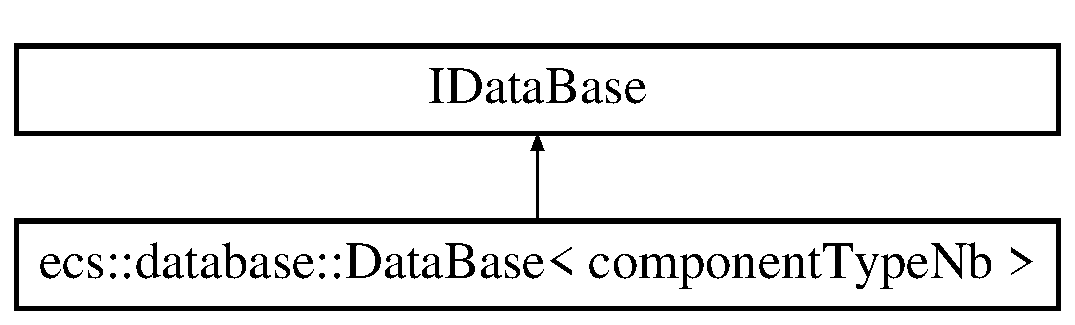
\includegraphics[height=2.000000cm]{d6/ddd/classecs_1_1database_1_1_data_base}
\end{center}
\end{figure}
\subsection*{Public Member Functions}
\begin{DoxyCompactItemize}
\item 
{\bf Data\+Base} (void)
\item 
{\bf Data\+Base} ({\bf Data\+Base} const \&)=delete
\item 
{\bf $\sim$\+Data\+Base} (void)
\item 
{\bf Data\+Base} \& {\bf operator=} ({\bf Data\+Base} const \&)=delete
\item 
ID$<$ Entity $>$ {\bf create\+Entity} (Entity\+Type const entity\+Type)
\item 
ID$<$ Entity $>$ {\bf create\+And\+Assemble\+Entity} (Entity\+Type const entity\+Type, Assembly\+Type const assembly\+Type)
\item 
ID$<$ Component $>$ {\bf create\+Component} (Component\+Type const component\+Type)
\item 
ID$<$ Component $>$ {\bf create\+And\+Bind\+Component} (Component\+Type const component\+Type, ID$<$ Entity $>$ const \&entity\+Id)
\end{DoxyCompactItemize}


\subsection{Constructor \& Destructor Documentation}
\label{classecs_1_1database_1_1_data_base_a871d8e2646bdd28a7798922028eac188} 
\index{ecs\+::database\+::\+Data\+Base@{ecs\+::database\+::\+Data\+Base}!Data\+Base@{Data\+Base}}
\index{Data\+Base@{Data\+Base}!ecs\+::database\+::\+Data\+Base@{ecs\+::database\+::\+Data\+Base}}
\subsubsection{Data\+Base()\hspace{0.1cm}{\footnotesize\ttfamily [1/2]}}
{\footnotesize\ttfamily template$<$unsigned const component\+Type\+Nb$>$ \\
{\bf ecs\+::database\+::\+Data\+Base}$<$ component\+Type\+Nb $>$\+::{\bf Data\+Base} (\begin{DoxyParamCaption}\item[{void}]{ }\end{DoxyParamCaption})}

\label{classecs_1_1database_1_1_data_base_a579413631c10476c036097b5eadb9721} 
\index{ecs\+::database\+::\+Data\+Base@{ecs\+::database\+::\+Data\+Base}!Data\+Base@{Data\+Base}}
\index{Data\+Base@{Data\+Base}!ecs\+::database\+::\+Data\+Base@{ecs\+::database\+::\+Data\+Base}}
\subsubsection{Data\+Base()\hspace{0.1cm}{\footnotesize\ttfamily [2/2]}}
{\footnotesize\ttfamily template$<$unsigned const component\+Type\+Nb$>$ \\
{\bf ecs\+::database\+::\+Data\+Base}$<$ component\+Type\+Nb $>$\+::{\bf Data\+Base} (\begin{DoxyParamCaption}\item[{{\bf Data\+Base}$<$ component\+Type\+Nb $>$ const \&}]{ }\end{DoxyParamCaption})\hspace{0.3cm}{\ttfamily [delete]}}

\label{classecs_1_1database_1_1_data_base_a8aa55d2b55636d8069802298d57755a1} 
\index{ecs\+::database\+::\+Data\+Base@{ecs\+::database\+::\+Data\+Base}!````~Data\+Base@{$\sim$\+Data\+Base}}
\index{````~Data\+Base@{$\sim$\+Data\+Base}!ecs\+::database\+::\+Data\+Base@{ecs\+::database\+::\+Data\+Base}}
\subsubsection{$\sim$\+Data\+Base()}
{\footnotesize\ttfamily template$<$unsigned const component\+Type\+Nb$>$ \\
{\bf ecs\+::database\+::\+Data\+Base}$<$ component\+Type\+Nb $>$\+::$\sim${\bf Data\+Base} (\begin{DoxyParamCaption}\item[{void}]{ }\end{DoxyParamCaption})}



\subsection{Member Function Documentation}
\label{classecs_1_1database_1_1_data_base_ad7cea6e99447ea681b8d8a666d13c134} 
\index{ecs\+::database\+::\+Data\+Base@{ecs\+::database\+::\+Data\+Base}!create\+And\+Assemble\+Entity@{create\+And\+Assemble\+Entity}}
\index{create\+And\+Assemble\+Entity@{create\+And\+Assemble\+Entity}!ecs\+::database\+::\+Data\+Base@{ecs\+::database\+::\+Data\+Base}}
\subsubsection{create\+And\+Assemble\+Entity()}
{\footnotesize\ttfamily template$<$unsigned const component\+Type\+Nb$>$ \\
ID$<$Entity$>$ {\bf ecs\+::database\+::\+Data\+Base}$<$ component\+Type\+Nb $>$\+::create\+And\+Assemble\+Entity (\begin{DoxyParamCaption}\item[{Entity\+Type const}]{entity\+Type,  }\item[{Assembly\+Type const}]{assembly\+Type }\end{DoxyParamCaption})}

\label{classecs_1_1database_1_1_data_base_a3cea49d97f99fbda75268c9ed979f4b8} 
\index{ecs\+::database\+::\+Data\+Base@{ecs\+::database\+::\+Data\+Base}!create\+And\+Bind\+Component@{create\+And\+Bind\+Component}}
\index{create\+And\+Bind\+Component@{create\+And\+Bind\+Component}!ecs\+::database\+::\+Data\+Base@{ecs\+::database\+::\+Data\+Base}}
\subsubsection{create\+And\+Bind\+Component()}
{\footnotesize\ttfamily template$<$unsigned const component\+Type\+Nb$>$ \\
ID$<$Component$>$ {\bf ecs\+::database\+::\+Data\+Base}$<$ component\+Type\+Nb $>$\+::create\+And\+Bind\+Component (\begin{DoxyParamCaption}\item[{Component\+Type const}]{component\+Type,  }\item[{ID$<$ Entity $>$ const \&}]{entity\+Id }\end{DoxyParamCaption})}

\label{classecs_1_1database_1_1_data_base_a6eb3c212e7e7b4accfe167c0606a4c0a} 
\index{ecs\+::database\+::\+Data\+Base@{ecs\+::database\+::\+Data\+Base}!create\+Component@{create\+Component}}
\index{create\+Component@{create\+Component}!ecs\+::database\+::\+Data\+Base@{ecs\+::database\+::\+Data\+Base}}
\subsubsection{create\+Component()}
{\footnotesize\ttfamily template$<$unsigned const component\+Type\+Nb$>$ \\
ID$<$Component$>$ {\bf ecs\+::database\+::\+Data\+Base}$<$ component\+Type\+Nb $>$\+::create\+Component (\begin{DoxyParamCaption}\item[{Component\+Type const}]{component\+Type }\end{DoxyParamCaption})}

\label{classecs_1_1database_1_1_data_base_aa2a54122ba4fbc1e3ec47b9c57a6b541} 
\index{ecs\+::database\+::\+Data\+Base@{ecs\+::database\+::\+Data\+Base}!create\+Entity@{create\+Entity}}
\index{create\+Entity@{create\+Entity}!ecs\+::database\+::\+Data\+Base@{ecs\+::database\+::\+Data\+Base}}
\subsubsection{create\+Entity()}
{\footnotesize\ttfamily template$<$unsigned const component\+Type\+Nb$>$ \\
ID$<$Entity$>$ {\bf ecs\+::database\+::\+Data\+Base}$<$ component\+Type\+Nb $>$\+::create\+Entity (\begin{DoxyParamCaption}\item[{Entity\+Type const}]{entity\+Type }\end{DoxyParamCaption})}

\label{classecs_1_1database_1_1_data_base_a5117ff72440665221fa33b91f8f61f64} 
\index{ecs\+::database\+::\+Data\+Base@{ecs\+::database\+::\+Data\+Base}!operator=@{operator=}}
\index{operator=@{operator=}!ecs\+::database\+::\+Data\+Base@{ecs\+::database\+::\+Data\+Base}}
\subsubsection{operator=()}
{\footnotesize\ttfamily template$<$unsigned const component\+Type\+Nb$>$ \\
{\bf Data\+Base}\& {\bf ecs\+::database\+::\+Data\+Base}$<$ component\+Type\+Nb $>$\+::operator= (\begin{DoxyParamCaption}\item[{{\bf Data\+Base}$<$ component\+Type\+Nb $>$ const \&}]{ }\end{DoxyParamCaption})\hspace{0.3cm}{\ttfamily [delete]}}



The documentation for this class was generated from the following file\+:\begin{DoxyCompactItemize}
\item 
inc/shared/{\bf Data\+Base.\+hpp}\end{DoxyCompactItemize}

\input{d7/ddf/classentity__component__system_1_1database_1_1_entity}
\input{d3/df7/structcompile__time_1_1_gen_index}
\input{d9/d2a/structcompile__time_1_1_gen_index_3_010_01_4}
\section{entity\+\_\+component\+\_\+system\+:\+:database\+:\+:ID$<$ T $>$ Class Template Reference}
\label{classentity__component__system_1_1database_1_1_i_d}\index{entity\+\_\+component\+\_\+system\+::database\+::\+I\+D$<$ T $>$@{entity\+\_\+component\+\_\+system\+::database\+::\+I\+D$<$ T $>$}}


{\ttfamily \#include $<$I\+Data\+Base.\+hpp$>$}

\subsection*{Public Member Functions}
\begin{DoxyCompactItemize}
\item 
{\bf ID} (unsigned const id)
\item 
{\bf ID} ({\bf ID}$<$ T $>$ const \&src)
\item 
{\bf ID} ({\bf ID}$<$ T $>$ \&\&src)
\item 
{\bf $\sim$\+ID} (void)
\item 
bool {\bf operator$<$} ({\bf ID}$<$ T $>$ const \&rhs) const
\item 
bool {\bf operator$>$} ({\bf ID}$<$ T $>$ const \&rhs) const
\item 
bool {\bf operator$<$=} ({\bf ID}$<$ T $>$ const \&rhs) const
\item 
bool {\bf operator$>$=} ({\bf ID}$<$ T $>$ const \&rhs) const
\item 
bool {\bf operator!=} ({\bf ID}$<$ T $>$ const \&rhs) const
\item 
bool {\bf operator==} ({\bf ID}$<$ T $>$ const \&rhs) const
\item 
{\bf ID}$<$ T $>$ \& {\bf operator=} ({\bf ID}$<$ T $>$ const \&src)
\item 
{\bf ID}$<$ T $>$ \& {\bf operator=} ({\bf ID}$<$ T $>$ \&\&src)
\end{DoxyCompactItemize}


\subsection{Constructor \& Destructor Documentation}
\label{classentity__component__system_1_1database_1_1_i_d_a3c6b323ed778d392cf6e9840f431310a} 
\index{entity\+\_\+component\+\_\+system\+::database\+::\+ID@{entity\+\_\+component\+\_\+system\+::database\+::\+ID}!ID@{ID}}
\index{ID@{ID}!entity\+\_\+component\+\_\+system\+::database\+::\+ID@{entity\+\_\+component\+\_\+system\+::database\+::\+ID}}
\subsubsection{I\+D()\hspace{0.1cm}{\footnotesize\ttfamily [1/3]}}
{\footnotesize\ttfamily template$<$typename T$>$ \\
{\bf entity\+\_\+component\+\_\+system\+::database\+::\+ID}$<$ T $>$\+::{\bf ID} (\begin{DoxyParamCaption}\item[{unsigned const}]{id }\end{DoxyParamCaption})\hspace{0.3cm}{\ttfamily [inline]}}

\label{classentity__component__system_1_1database_1_1_i_d_aca2a1c239a78455fbcbe0b2077ad7ece} 
\index{entity\+\_\+component\+\_\+system\+::database\+::\+ID@{entity\+\_\+component\+\_\+system\+::database\+::\+ID}!ID@{ID}}
\index{ID@{ID}!entity\+\_\+component\+\_\+system\+::database\+::\+ID@{entity\+\_\+component\+\_\+system\+::database\+::\+ID}}
\subsubsection{I\+D()\hspace{0.1cm}{\footnotesize\ttfamily [2/3]}}
{\footnotesize\ttfamily template$<$typename T$>$ \\
{\bf entity\+\_\+component\+\_\+system\+::database\+::\+ID}$<$ T $>$\+::{\bf ID} (\begin{DoxyParamCaption}\item[{{\bf ID}$<$ T $>$ const \&}]{src }\end{DoxyParamCaption})\hspace{0.3cm}{\ttfamily [inline]}}

\label{classentity__component__system_1_1database_1_1_i_d_ac236fcdaf32bed1990eff6183a5873b8} 
\index{entity\+\_\+component\+\_\+system\+::database\+::\+ID@{entity\+\_\+component\+\_\+system\+::database\+::\+ID}!ID@{ID}}
\index{ID@{ID}!entity\+\_\+component\+\_\+system\+::database\+::\+ID@{entity\+\_\+component\+\_\+system\+::database\+::\+ID}}
\subsubsection{I\+D()\hspace{0.1cm}{\footnotesize\ttfamily [3/3]}}
{\footnotesize\ttfamily template$<$typename T$>$ \\
{\bf entity\+\_\+component\+\_\+system\+::database\+::\+ID}$<$ T $>$\+::{\bf ID} (\begin{DoxyParamCaption}\item[{{\bf ID}$<$ T $>$ \&\&}]{src }\end{DoxyParamCaption})\hspace{0.3cm}{\ttfamily [inline]}}

\label{classentity__component__system_1_1database_1_1_i_d_aa0b62c76e72f26fc4b293a0694cd7978} 
\index{entity\+\_\+component\+\_\+system\+::database\+::\+ID@{entity\+\_\+component\+\_\+system\+::database\+::\+ID}!````~ID@{$\sim$\+ID}}
\index{````~ID@{$\sim$\+ID}!entity\+\_\+component\+\_\+system\+::database\+::\+ID@{entity\+\_\+component\+\_\+system\+::database\+::\+ID}}
\subsubsection{$\sim$\+I\+D()}
{\footnotesize\ttfamily template$<$typename T$>$ \\
{\bf entity\+\_\+component\+\_\+system\+::database\+::\+ID}$<$ T $>$\+::$\sim${\bf ID} (\begin{DoxyParamCaption}\item[{void}]{ }\end{DoxyParamCaption})\hspace{0.3cm}{\ttfamily [inline]}}



\subsection{Member Function Documentation}
\label{classentity__component__system_1_1database_1_1_i_d_a3523797fc895560d5df63ab485776c6f} 
\index{entity\+\_\+component\+\_\+system\+::database\+::\+ID@{entity\+\_\+component\+\_\+system\+::database\+::\+ID}!operator"!=@{operator"!=}}
\index{operator"!=@{operator"!=}!entity\+\_\+component\+\_\+system\+::database\+::\+ID@{entity\+\_\+component\+\_\+system\+::database\+::\+ID}}
\subsubsection{operator"!=()}
{\footnotesize\ttfamily template$<$typename T$>$ \\
bool {\bf entity\+\_\+component\+\_\+system\+::database\+::\+ID}$<$ T $>$\+::operator!= (\begin{DoxyParamCaption}\item[{{\bf ID}$<$ T $>$ const \&}]{rhs }\end{DoxyParamCaption}) const\hspace{0.3cm}{\ttfamily [inline]}}

\label{classentity__component__system_1_1database_1_1_i_d_a4c7c49f86a944e387984697530cbdb6d} 
\index{entity\+\_\+component\+\_\+system\+::database\+::\+ID@{entity\+\_\+component\+\_\+system\+::database\+::\+ID}!operator$<$@{operator$<$}}
\index{operator$<$@{operator$<$}!entity\+\_\+component\+\_\+system\+::database\+::\+ID@{entity\+\_\+component\+\_\+system\+::database\+::\+ID}}
\subsubsection{operator$<$()}
{\footnotesize\ttfamily template$<$typename T$>$ \\
bool {\bf entity\+\_\+component\+\_\+system\+::database\+::\+ID}$<$ T $>$\+::operator$<$ (\begin{DoxyParamCaption}\item[{{\bf ID}$<$ T $>$ const \&}]{rhs }\end{DoxyParamCaption}) const\hspace{0.3cm}{\ttfamily [inline]}}

\label{classentity__component__system_1_1database_1_1_i_d_ad9f2a2ee834a135026a2c8beb611fb15} 
\index{entity\+\_\+component\+\_\+system\+::database\+::\+ID@{entity\+\_\+component\+\_\+system\+::database\+::\+ID}!operator$<$=@{operator$<$=}}
\index{operator$<$=@{operator$<$=}!entity\+\_\+component\+\_\+system\+::database\+::\+ID@{entity\+\_\+component\+\_\+system\+::database\+::\+ID}}
\subsubsection{operator$<$=()}
{\footnotesize\ttfamily template$<$typename T$>$ \\
bool {\bf entity\+\_\+component\+\_\+system\+::database\+::\+ID}$<$ T $>$\+::operator$<$= (\begin{DoxyParamCaption}\item[{{\bf ID}$<$ T $>$ const \&}]{rhs }\end{DoxyParamCaption}) const\hspace{0.3cm}{\ttfamily [inline]}}

\label{classentity__component__system_1_1database_1_1_i_d_a0a6747e60880a92dff37ebb78f785085} 
\index{entity\+\_\+component\+\_\+system\+::database\+::\+ID@{entity\+\_\+component\+\_\+system\+::database\+::\+ID}!operator=@{operator=}}
\index{operator=@{operator=}!entity\+\_\+component\+\_\+system\+::database\+::\+ID@{entity\+\_\+component\+\_\+system\+::database\+::\+ID}}
\subsubsection{operator=()\hspace{0.1cm}{\footnotesize\ttfamily [1/2]}}
{\footnotesize\ttfamily template$<$typename T$>$ \\
{\bf ID}$<$T$>$\& {\bf entity\+\_\+component\+\_\+system\+::database\+::\+ID}$<$ T $>$\+::operator= (\begin{DoxyParamCaption}\item[{{\bf ID}$<$ T $>$ const \&}]{src }\end{DoxyParamCaption})\hspace{0.3cm}{\ttfamily [inline]}}

\label{classentity__component__system_1_1database_1_1_i_d_ab15bd244cdf0ff98107cecd99c02c888} 
\index{entity\+\_\+component\+\_\+system\+::database\+::\+ID@{entity\+\_\+component\+\_\+system\+::database\+::\+ID}!operator=@{operator=}}
\index{operator=@{operator=}!entity\+\_\+component\+\_\+system\+::database\+::\+ID@{entity\+\_\+component\+\_\+system\+::database\+::\+ID}}
\subsubsection{operator=()\hspace{0.1cm}{\footnotesize\ttfamily [2/2]}}
{\footnotesize\ttfamily template$<$typename T$>$ \\
{\bf ID}$<$T$>$\& {\bf entity\+\_\+component\+\_\+system\+::database\+::\+ID}$<$ T $>$\+::operator= (\begin{DoxyParamCaption}\item[{{\bf ID}$<$ T $>$ \&\&}]{src }\end{DoxyParamCaption})\hspace{0.3cm}{\ttfamily [inline]}}

\label{classentity__component__system_1_1database_1_1_i_d_ad64e6a0020d064586fe5d95a8b511305} 
\index{entity\+\_\+component\+\_\+system\+::database\+::\+ID@{entity\+\_\+component\+\_\+system\+::database\+::\+ID}!operator==@{operator==}}
\index{operator==@{operator==}!entity\+\_\+component\+\_\+system\+::database\+::\+ID@{entity\+\_\+component\+\_\+system\+::database\+::\+ID}}
\subsubsection{operator==()}
{\footnotesize\ttfamily template$<$typename T$>$ \\
bool {\bf entity\+\_\+component\+\_\+system\+::database\+::\+ID}$<$ T $>$\+::operator== (\begin{DoxyParamCaption}\item[{{\bf ID}$<$ T $>$ const \&}]{rhs }\end{DoxyParamCaption}) const\hspace{0.3cm}{\ttfamily [inline]}}

\label{classentity__component__system_1_1database_1_1_i_d_a3eea25166ccb0ef7a37a7299ac486072} 
\index{entity\+\_\+component\+\_\+system\+::database\+::\+ID@{entity\+\_\+component\+\_\+system\+::database\+::\+ID}!operator$>$@{operator$>$}}
\index{operator$>$@{operator$>$}!entity\+\_\+component\+\_\+system\+::database\+::\+ID@{entity\+\_\+component\+\_\+system\+::database\+::\+ID}}
\subsubsection{operator$>$()}
{\footnotesize\ttfamily template$<$typename T$>$ \\
bool {\bf entity\+\_\+component\+\_\+system\+::database\+::\+ID}$<$ T $>$\+::operator$>$ (\begin{DoxyParamCaption}\item[{{\bf ID}$<$ T $>$ const \&}]{rhs }\end{DoxyParamCaption}) const\hspace{0.3cm}{\ttfamily [inline]}}

\label{classentity__component__system_1_1database_1_1_i_d_a18013373a4e7fe43ba7cb1e561731495} 
\index{entity\+\_\+component\+\_\+system\+::database\+::\+ID@{entity\+\_\+component\+\_\+system\+::database\+::\+ID}!operator$>$=@{operator$>$=}}
\index{operator$>$=@{operator$>$=}!entity\+\_\+component\+\_\+system\+::database\+::\+ID@{entity\+\_\+component\+\_\+system\+::database\+::\+ID}}
\subsubsection{operator$>$=()}
{\footnotesize\ttfamily template$<$typename T$>$ \\
bool {\bf entity\+\_\+component\+\_\+system\+::database\+::\+ID}$<$ T $>$\+::operator$>$= (\begin{DoxyParamCaption}\item[{{\bf ID}$<$ T $>$ const \&}]{rhs }\end{DoxyParamCaption}) const\hspace{0.3cm}{\ttfamily [inline]}}



The documentation for this class was generated from the following file\+:\begin{DoxyCompactItemize}
\item 
inc/shared/{\bf I\+Data\+Base.\+hpp}\end{DoxyCompactItemize}

\section{entity\+\_\+component\+\_\+system\+:\+:database\+:\+:I\+Data\+Base$<$ Entity\+Type, Component\+Type, Assembly\+Type $>$ Class Template Reference}
\label{classentity__component__system_1_1database_1_1_i_data_base}\index{entity\+\_\+component\+\_\+system\+::database\+::\+I\+Data\+Base$<$ Entity\+Type, Component\+Type, Assembly\+Type $>$@{entity\+\_\+component\+\_\+system\+::database\+::\+I\+Data\+Base$<$ Entity\+Type, Component\+Type, Assembly\+Type $>$}}


{\ttfamily \#include $<$I\+Data\+Base.\+hpp$>$}

\subsection*{Public Member Functions}
\begin{DoxyCompactItemize}
\item 
virtual {\bf $\sim$\+I\+Data\+Base} (void)
\item 
virtual {\bf ID}$<$ Entity $>$ {\bf create\+Entity} (Entity\+Type const entity\+Type)=0
\item 
virtual {\bf ID}$<$ Entity $>$ {\bf create\+And\+Assemble\+Entity} (Entity\+Type const entity\+Type, Assembly\+Type const assembly\+Type)=0
\item 
virtual {\bf ID}$<$ Component $>$ {\bf create\+Component} (Component\+Type const component\+Type, unsigned const attr\+Nb)=0
\item 
virtual {\bf ID}$<$ Component $>$ {\bf create\+And\+Bind\+Component} (Component\+Type const component\+Type, {\bf ID}$<$ Entity $>$ const \&entity\+Id)=0
\item 
virtual void {\bf bind\+Component\+To\+Assembly} (Assembly\+Type const assembly\+Type, Component\+Type const component\+Type)=0
\item 
virtual {\bf ID}$<$ Component $>$ {\bf bind\+Component\+To\+Entity} ({\bf ID}$<$ Entity $>$ const \&entity\+Id, Component\+Type const component\+Type, {\bf ID}$<$ Component $>$ const \&component\+Id)=0
\item 
virtual stde\+::any {\bf get\+Entity} ({\bf ID}$<$ Entity $>$ const \&id, std\+::list$<$ Component\+Type $>$ const \&components) const =0
\item 
virtual stde\+::any {\bf get\+Component\+In\+Entity} ({\bf ID}$<$ Entity $>$ const \&id, Component\+Type const component\+Type) const =0
\item 
virtual stde\+::any {\bf get\+All\+Entities} (Entity\+Type const entity\+Type) const =0
\item 
virtual stde\+::any {\bf get\+Entity\+With\+Component\+Equal\+To} (Component\+Type const component\+Type, stde\+::any const \&value) const =0
\item 
virtual void {\bf set\+Entity} ({\bf ID}$<$ Entity $>$ const \&id, stde\+::any const \&entity)=0
\item 
virtual void {\bf set\+Entities} (std\+::vector$<$ std\+::pair$<$ {\bf ID}$<$ Entity $>$, stde\+::any $>$$>$ const \&entities)=0
\item 
virtual void {\bf set\+Component} ({\bf ID}$<$ Entity $>$ const \&entity\+Id, Component\+Type const component\+Type, stde\+::any const \&component)=0
\end{DoxyCompactItemize}


\subsection{Constructor \& Destructor Documentation}
\label{classentity__component__system_1_1database_1_1_i_data_base_abcbd6e03736ab22392af6a5af784744e} 
\index{entity\+\_\+component\+\_\+system\+::database\+::\+I\+Data\+Base@{entity\+\_\+component\+\_\+system\+::database\+::\+I\+Data\+Base}!````~I\+Data\+Base@{$\sim$\+I\+Data\+Base}}
\index{````~I\+Data\+Base@{$\sim$\+I\+Data\+Base}!entity\+\_\+component\+\_\+system\+::database\+::\+I\+Data\+Base@{entity\+\_\+component\+\_\+system\+::database\+::\+I\+Data\+Base}}
\subsubsection{$\sim$\+I\+Data\+Base()}
{\footnotesize\ttfamily template$<$typename Entity\+Type , typename Component\+Type , typename Assembly\+Type $>$ \\
virtual {\bf entity\+\_\+component\+\_\+system\+::database\+::\+I\+Data\+Base}$<$ Entity\+Type, Component\+Type, Assembly\+Type $>$\+::$\sim${\bf I\+Data\+Base} (\begin{DoxyParamCaption}\item[{void}]{ }\end{DoxyParamCaption})\hspace{0.3cm}{\ttfamily [inline]}, {\ttfamily [virtual]}}



\subsection{Member Function Documentation}
\label{classentity__component__system_1_1database_1_1_i_data_base_a6f9eb76615a1bea6d93f562ca2380bae} 
\index{entity\+\_\+component\+\_\+system\+::database\+::\+I\+Data\+Base@{entity\+\_\+component\+\_\+system\+::database\+::\+I\+Data\+Base}!bind\+Component\+To\+Assembly@{bind\+Component\+To\+Assembly}}
\index{bind\+Component\+To\+Assembly@{bind\+Component\+To\+Assembly}!entity\+\_\+component\+\_\+system\+::database\+::\+I\+Data\+Base@{entity\+\_\+component\+\_\+system\+::database\+::\+I\+Data\+Base}}
\subsubsection{bind\+Component\+To\+Assembly()}
{\footnotesize\ttfamily template$<$typename Entity\+Type , typename Component\+Type , typename Assembly\+Type $>$ \\
virtual void {\bf entity\+\_\+component\+\_\+system\+::database\+::\+I\+Data\+Base}$<$ Entity\+Type, Component\+Type, Assembly\+Type $>$\+::bind\+Component\+To\+Assembly (\begin{DoxyParamCaption}\item[{Assembly\+Type const}]{assembly\+Type,  }\item[{Component\+Type const}]{component\+Type }\end{DoxyParamCaption})\hspace{0.3cm}{\ttfamily [pure virtual]}}

\label{classentity__component__system_1_1database_1_1_i_data_base_a3fa3416dbb90294924923df7a67db356} 
\index{entity\+\_\+component\+\_\+system\+::database\+::\+I\+Data\+Base@{entity\+\_\+component\+\_\+system\+::database\+::\+I\+Data\+Base}!bind\+Component\+To\+Entity@{bind\+Component\+To\+Entity}}
\index{bind\+Component\+To\+Entity@{bind\+Component\+To\+Entity}!entity\+\_\+component\+\_\+system\+::database\+::\+I\+Data\+Base@{entity\+\_\+component\+\_\+system\+::database\+::\+I\+Data\+Base}}
\subsubsection{bind\+Component\+To\+Entity()}
{\footnotesize\ttfamily template$<$typename Entity\+Type , typename Component\+Type , typename Assembly\+Type $>$ \\
virtual {\bf ID}$<$Component$>$ {\bf entity\+\_\+component\+\_\+system\+::database\+::\+I\+Data\+Base}$<$ Entity\+Type, Component\+Type, Assembly\+Type $>$\+::bind\+Component\+To\+Entity (\begin{DoxyParamCaption}\item[{{\bf ID}$<$ Entity $>$ const \&}]{entity\+Id,  }\item[{Component\+Type const}]{component\+Type,  }\item[{{\bf ID}$<$ Component $>$ const \&}]{component\+Id }\end{DoxyParamCaption})\hspace{0.3cm}{\ttfamily [pure virtual]}}

\label{classentity__component__system_1_1database_1_1_i_data_base_a41c7ed5f04ac166e142878e32ae5e3e5} 
\index{entity\+\_\+component\+\_\+system\+::database\+::\+I\+Data\+Base@{entity\+\_\+component\+\_\+system\+::database\+::\+I\+Data\+Base}!create\+And\+Assemble\+Entity@{create\+And\+Assemble\+Entity}}
\index{create\+And\+Assemble\+Entity@{create\+And\+Assemble\+Entity}!entity\+\_\+component\+\_\+system\+::database\+::\+I\+Data\+Base@{entity\+\_\+component\+\_\+system\+::database\+::\+I\+Data\+Base}}
\subsubsection{create\+And\+Assemble\+Entity()}
{\footnotesize\ttfamily template$<$typename Entity\+Type , typename Component\+Type , typename Assembly\+Type $>$ \\
virtual {\bf ID}$<$Entity$>$ {\bf entity\+\_\+component\+\_\+system\+::database\+::\+I\+Data\+Base}$<$ Entity\+Type, Component\+Type, Assembly\+Type $>$\+::create\+And\+Assemble\+Entity (\begin{DoxyParamCaption}\item[{Entity\+Type const}]{entity\+Type,  }\item[{Assembly\+Type const}]{assembly\+Type }\end{DoxyParamCaption})\hspace{0.3cm}{\ttfamily [pure virtual]}}

\label{classentity__component__system_1_1database_1_1_i_data_base_ac3b147adcd7971a7925affabb81ee6bb} 
\index{entity\+\_\+component\+\_\+system\+::database\+::\+I\+Data\+Base@{entity\+\_\+component\+\_\+system\+::database\+::\+I\+Data\+Base}!create\+And\+Bind\+Component@{create\+And\+Bind\+Component}}
\index{create\+And\+Bind\+Component@{create\+And\+Bind\+Component}!entity\+\_\+component\+\_\+system\+::database\+::\+I\+Data\+Base@{entity\+\_\+component\+\_\+system\+::database\+::\+I\+Data\+Base}}
\subsubsection{create\+And\+Bind\+Component()}
{\footnotesize\ttfamily template$<$typename Entity\+Type , typename Component\+Type , typename Assembly\+Type $>$ \\
virtual {\bf ID}$<$Component$>$ {\bf entity\+\_\+component\+\_\+system\+::database\+::\+I\+Data\+Base}$<$ Entity\+Type, Component\+Type, Assembly\+Type $>$\+::create\+And\+Bind\+Component (\begin{DoxyParamCaption}\item[{Component\+Type const}]{component\+Type,  }\item[{{\bf ID}$<$ Entity $>$ const \&}]{entity\+Id }\end{DoxyParamCaption})\hspace{0.3cm}{\ttfamily [pure virtual]}}

\label{classentity__component__system_1_1database_1_1_i_data_base_a7015be247d4bbc4497c6965c7f29af2a} 
\index{entity\+\_\+component\+\_\+system\+::database\+::\+I\+Data\+Base@{entity\+\_\+component\+\_\+system\+::database\+::\+I\+Data\+Base}!create\+Component@{create\+Component}}
\index{create\+Component@{create\+Component}!entity\+\_\+component\+\_\+system\+::database\+::\+I\+Data\+Base@{entity\+\_\+component\+\_\+system\+::database\+::\+I\+Data\+Base}}
\subsubsection{create\+Component()}
{\footnotesize\ttfamily template$<$typename Entity\+Type , typename Component\+Type , typename Assembly\+Type $>$ \\
virtual {\bf ID}$<$Component$>$ {\bf entity\+\_\+component\+\_\+system\+::database\+::\+I\+Data\+Base}$<$ Entity\+Type, Component\+Type, Assembly\+Type $>$\+::create\+Component (\begin{DoxyParamCaption}\item[{Component\+Type const}]{component\+Type,  }\item[{unsigned const}]{attr\+Nb }\end{DoxyParamCaption})\hspace{0.3cm}{\ttfamily [pure virtual]}}

\label{classentity__component__system_1_1database_1_1_i_data_base_ade6b15fec900be773f3ef01f04dc1bb2} 
\index{entity\+\_\+component\+\_\+system\+::database\+::\+I\+Data\+Base@{entity\+\_\+component\+\_\+system\+::database\+::\+I\+Data\+Base}!create\+Entity@{create\+Entity}}
\index{create\+Entity@{create\+Entity}!entity\+\_\+component\+\_\+system\+::database\+::\+I\+Data\+Base@{entity\+\_\+component\+\_\+system\+::database\+::\+I\+Data\+Base}}
\subsubsection{create\+Entity()}
{\footnotesize\ttfamily template$<$typename Entity\+Type , typename Component\+Type , typename Assembly\+Type $>$ \\
virtual {\bf ID}$<$Entity$>$ {\bf entity\+\_\+component\+\_\+system\+::database\+::\+I\+Data\+Base}$<$ Entity\+Type, Component\+Type, Assembly\+Type $>$\+::create\+Entity (\begin{DoxyParamCaption}\item[{Entity\+Type const}]{entity\+Type }\end{DoxyParamCaption})\hspace{0.3cm}{\ttfamily [pure virtual]}}

\label{classentity__component__system_1_1database_1_1_i_data_base_abad727d40380efadf24294e9ab1e5465} 
\index{entity\+\_\+component\+\_\+system\+::database\+::\+I\+Data\+Base@{entity\+\_\+component\+\_\+system\+::database\+::\+I\+Data\+Base}!get\+All\+Entities@{get\+All\+Entities}}
\index{get\+All\+Entities@{get\+All\+Entities}!entity\+\_\+component\+\_\+system\+::database\+::\+I\+Data\+Base@{entity\+\_\+component\+\_\+system\+::database\+::\+I\+Data\+Base}}
\subsubsection{get\+All\+Entities()}
{\footnotesize\ttfamily template$<$typename Entity\+Type , typename Component\+Type , typename Assembly\+Type $>$ \\
virtual stde\+::any {\bf entity\+\_\+component\+\_\+system\+::database\+::\+I\+Data\+Base}$<$ Entity\+Type, Component\+Type, Assembly\+Type $>$\+::get\+All\+Entities (\begin{DoxyParamCaption}\item[{Entity\+Type const}]{entity\+Type }\end{DoxyParamCaption}) const\hspace{0.3cm}{\ttfamily [pure virtual]}}

\label{classentity__component__system_1_1database_1_1_i_data_base_a29002a97151f394a59e3e9e9ce72ea27} 
\index{entity\+\_\+component\+\_\+system\+::database\+::\+I\+Data\+Base@{entity\+\_\+component\+\_\+system\+::database\+::\+I\+Data\+Base}!get\+Component\+In\+Entity@{get\+Component\+In\+Entity}}
\index{get\+Component\+In\+Entity@{get\+Component\+In\+Entity}!entity\+\_\+component\+\_\+system\+::database\+::\+I\+Data\+Base@{entity\+\_\+component\+\_\+system\+::database\+::\+I\+Data\+Base}}
\subsubsection{get\+Component\+In\+Entity()}
{\footnotesize\ttfamily template$<$typename Entity\+Type , typename Component\+Type , typename Assembly\+Type $>$ \\
virtual stde\+::any {\bf entity\+\_\+component\+\_\+system\+::database\+::\+I\+Data\+Base}$<$ Entity\+Type, Component\+Type, Assembly\+Type $>$\+::get\+Component\+In\+Entity (\begin{DoxyParamCaption}\item[{{\bf ID}$<$ Entity $>$ const \&}]{id,  }\item[{Component\+Type const}]{component\+Type }\end{DoxyParamCaption}) const\hspace{0.3cm}{\ttfamily [pure virtual]}}

\label{classentity__component__system_1_1database_1_1_i_data_base_a98eadaccbb949f8f6cb77e4469e992ed} 
\index{entity\+\_\+component\+\_\+system\+::database\+::\+I\+Data\+Base@{entity\+\_\+component\+\_\+system\+::database\+::\+I\+Data\+Base}!get\+Entity@{get\+Entity}}
\index{get\+Entity@{get\+Entity}!entity\+\_\+component\+\_\+system\+::database\+::\+I\+Data\+Base@{entity\+\_\+component\+\_\+system\+::database\+::\+I\+Data\+Base}}
\subsubsection{get\+Entity()}
{\footnotesize\ttfamily template$<$typename Entity\+Type , typename Component\+Type , typename Assembly\+Type $>$ \\
virtual stde\+::any {\bf entity\+\_\+component\+\_\+system\+::database\+::\+I\+Data\+Base}$<$ Entity\+Type, Component\+Type, Assembly\+Type $>$\+::get\+Entity (\begin{DoxyParamCaption}\item[{{\bf ID}$<$ Entity $>$ const \&}]{id,  }\item[{std\+::list$<$ Component\+Type $>$ const \&}]{components }\end{DoxyParamCaption}) const\hspace{0.3cm}{\ttfamily [pure virtual]}}

\label{classentity__component__system_1_1database_1_1_i_data_base_a2c492e0043e6947e65477077b4bb5dd5} 
\index{entity\+\_\+component\+\_\+system\+::database\+::\+I\+Data\+Base@{entity\+\_\+component\+\_\+system\+::database\+::\+I\+Data\+Base}!get\+Entity\+With\+Component\+Equal\+To@{get\+Entity\+With\+Component\+Equal\+To}}
\index{get\+Entity\+With\+Component\+Equal\+To@{get\+Entity\+With\+Component\+Equal\+To}!entity\+\_\+component\+\_\+system\+::database\+::\+I\+Data\+Base@{entity\+\_\+component\+\_\+system\+::database\+::\+I\+Data\+Base}}
\subsubsection{get\+Entity\+With\+Component\+Equal\+To()}
{\footnotesize\ttfamily template$<$typename Entity\+Type , typename Component\+Type , typename Assembly\+Type $>$ \\
virtual stde\+::any {\bf entity\+\_\+component\+\_\+system\+::database\+::\+I\+Data\+Base}$<$ Entity\+Type, Component\+Type, Assembly\+Type $>$\+::get\+Entity\+With\+Component\+Equal\+To (\begin{DoxyParamCaption}\item[{Component\+Type const}]{component\+Type,  }\item[{stde\+::any const \&}]{value }\end{DoxyParamCaption}) const\hspace{0.3cm}{\ttfamily [pure virtual]}}

\label{classentity__component__system_1_1database_1_1_i_data_base_ae91982e5f21800ae984fc8e903dee7af} 
\index{entity\+\_\+component\+\_\+system\+::database\+::\+I\+Data\+Base@{entity\+\_\+component\+\_\+system\+::database\+::\+I\+Data\+Base}!set\+Component@{set\+Component}}
\index{set\+Component@{set\+Component}!entity\+\_\+component\+\_\+system\+::database\+::\+I\+Data\+Base@{entity\+\_\+component\+\_\+system\+::database\+::\+I\+Data\+Base}}
\subsubsection{set\+Component()}
{\footnotesize\ttfamily template$<$typename Entity\+Type , typename Component\+Type , typename Assembly\+Type $>$ \\
virtual void {\bf entity\+\_\+component\+\_\+system\+::database\+::\+I\+Data\+Base}$<$ Entity\+Type, Component\+Type, Assembly\+Type $>$\+::set\+Component (\begin{DoxyParamCaption}\item[{{\bf ID}$<$ Entity $>$ const \&}]{entity\+Id,  }\item[{Component\+Type const}]{component\+Type,  }\item[{stde\+::any const \&}]{component }\end{DoxyParamCaption})\hspace{0.3cm}{\ttfamily [pure virtual]}}

\label{classentity__component__system_1_1database_1_1_i_data_base_a5da3a689eaa89a9095eb3f6e0ed30e12} 
\index{entity\+\_\+component\+\_\+system\+::database\+::\+I\+Data\+Base@{entity\+\_\+component\+\_\+system\+::database\+::\+I\+Data\+Base}!set\+Entities@{set\+Entities}}
\index{set\+Entities@{set\+Entities}!entity\+\_\+component\+\_\+system\+::database\+::\+I\+Data\+Base@{entity\+\_\+component\+\_\+system\+::database\+::\+I\+Data\+Base}}
\subsubsection{set\+Entities()}
{\footnotesize\ttfamily template$<$typename Entity\+Type , typename Component\+Type , typename Assembly\+Type $>$ \\
virtual void {\bf entity\+\_\+component\+\_\+system\+::database\+::\+I\+Data\+Base}$<$ Entity\+Type, Component\+Type, Assembly\+Type $>$\+::set\+Entities (\begin{DoxyParamCaption}\item[{std\+::vector$<$ std\+::pair$<$ {\bf ID}$<$ Entity $>$, stde\+::any $>$$>$ const \&}]{entities }\end{DoxyParamCaption})\hspace{0.3cm}{\ttfamily [pure virtual]}}

\label{classentity__component__system_1_1database_1_1_i_data_base_afb4f8e2f3979eaf552589c9c97b03e36} 
\index{entity\+\_\+component\+\_\+system\+::database\+::\+I\+Data\+Base@{entity\+\_\+component\+\_\+system\+::database\+::\+I\+Data\+Base}!set\+Entity@{set\+Entity}}
\index{set\+Entity@{set\+Entity}!entity\+\_\+component\+\_\+system\+::database\+::\+I\+Data\+Base@{entity\+\_\+component\+\_\+system\+::database\+::\+I\+Data\+Base}}
\subsubsection{set\+Entity()}
{\footnotesize\ttfamily template$<$typename Entity\+Type , typename Component\+Type , typename Assembly\+Type $>$ \\
virtual void {\bf entity\+\_\+component\+\_\+system\+::database\+::\+I\+Data\+Base}$<$ Entity\+Type, Component\+Type, Assembly\+Type $>$\+::set\+Entity (\begin{DoxyParamCaption}\item[{{\bf ID}$<$ Entity $>$ const \&}]{id,  }\item[{stde\+::any const \&}]{entity }\end{DoxyParamCaption})\hspace{0.3cm}{\ttfamily [pure virtual]}}



The documentation for this class was generated from the following file\+:\begin{DoxyCompactItemize}
\item 
inc/shared/{\bf I\+Data\+Base.\+hpp}\end{DoxyCompactItemize}

\input{dd/d34/classentity__component__system_1_1_identifier_found}
\section{entity\+\_\+component\+\_\+system\+:\+:Identifier\+Not\+Found Class Reference}
\label{classentity__component__system_1_1_identifier_not_found}\index{entity\+\_\+component\+\_\+system\+::\+Identifier\+Not\+Found@{entity\+\_\+component\+\_\+system\+::\+Identifier\+Not\+Found}}


Exception class Raised when a component / attribute is not found while accessing it from an entity / component, respectively.  




{\ttfamily \#include $<$Identifier\+Not\+Found.\+hpp$>$}

Inheritance diagram for entity\+\_\+component\+\_\+system\+:\+:Identifier\+Not\+Found\+:\begin{figure}[H]
\begin{center}
\leavevmode
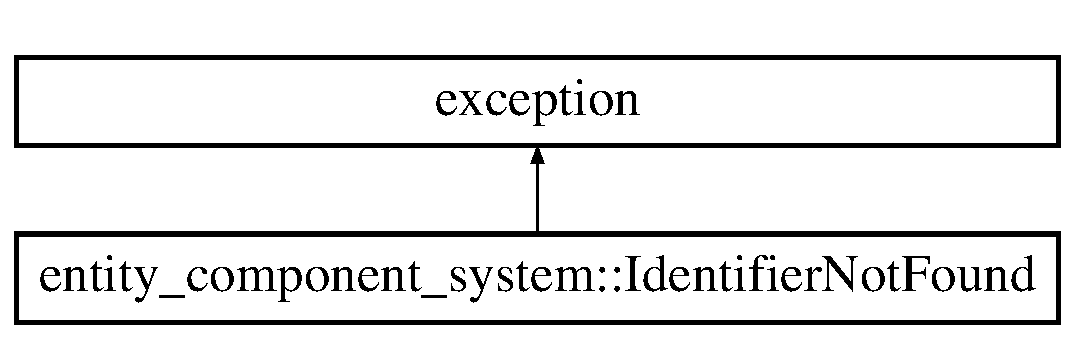
\includegraphics[height=2.000000cm]{d0/d3f/classentity__component__system_1_1_identifier_not_found}
\end{center}
\end{figure}
\subsection*{Public Member Functions}
\begin{DoxyCompactItemize}
\item 
{\bf Identifier\+Not\+Found} (std\+::string const \&id) noexcept
\begin{DoxyCompactList}\small\item\em Constructor. \end{DoxyCompactList}\item 
char const  $\ast$ {\bf what} (void) const noexcept
\begin{DoxyCompactList}\small\item\em get the error message \end{DoxyCompactList}\end{DoxyCompactItemize}


\subsection{Detailed Description}
Exception class Raised when a component / attribute is not found while accessing it from an entity / component, respectively. 

\subsection{Constructor \& Destructor Documentation}
\label{classentity__component__system_1_1_identifier_not_found_a2f9ffc48c910bee477f48dcd6f577475} 
\index{entity\+\_\+component\+\_\+system\+::\+Identifier\+Not\+Found@{entity\+\_\+component\+\_\+system\+::\+Identifier\+Not\+Found}!Identifier\+Not\+Found@{Identifier\+Not\+Found}}
\index{Identifier\+Not\+Found@{Identifier\+Not\+Found}!entity\+\_\+component\+\_\+system\+::\+Identifier\+Not\+Found@{entity\+\_\+component\+\_\+system\+::\+Identifier\+Not\+Found}}
\subsubsection{Identifier\+Not\+Found()}
{\footnotesize\ttfamily entity\+\_\+component\+\_\+system\+::\+Identifier\+Not\+Found\+::\+Identifier\+Not\+Found (\begin{DoxyParamCaption}\item[{std\+::string const \&}]{id }\end{DoxyParamCaption})\hspace{0.3cm}{\ttfamily [noexcept]}}



Constructor. 



\subsection{Member Function Documentation}
\label{classentity__component__system_1_1_identifier_not_found_ae06dfcab94cfb77e21e4eaa0b893ea3a} 
\index{entity\+\_\+component\+\_\+system\+::\+Identifier\+Not\+Found@{entity\+\_\+component\+\_\+system\+::\+Identifier\+Not\+Found}!what@{what}}
\index{what@{what}!entity\+\_\+component\+\_\+system\+::\+Identifier\+Not\+Found@{entity\+\_\+component\+\_\+system\+::\+Identifier\+Not\+Found}}
\subsubsection{what()}
{\footnotesize\ttfamily char const  $\ast$ entity\+\_\+component\+\_\+system\+::\+Identifier\+Not\+Found\+::what (\begin{DoxyParamCaption}\item[{void}]{ }\end{DoxyParamCaption}) const\hspace{0.3cm}{\ttfamily [noexcept]}}



get the error message 

\begin{DoxyReturn}{Returns}
a pointer to the constant error message 
\end{DoxyReturn}


The documentation for this class was generated from the following files\+:\begin{DoxyCompactItemize}
\item 
inc/shared/{\bf Identifier\+Not\+Found.\+hpp}\item 
src/shared/{\bf Identifier\+Not\+Found.\+cpp}\end{DoxyCompactItemize}

\input{d7/dc1/structcompile__time_1_1_index}
\input{da/da7/classentity__component__system_1_1entity_1_1_r_t_entity}
\input{d3/d70/structcompile__time_1_1_types_wrapper}
\input{d4/d3c/structcompile__time_1_1_wrapper}
\chapter{File Documentation}
\input{db/d34/_bad_type_8hpp}
\input{dc/d76/_compile_time_8hpp}
\section{inc/shared/\+Component.hpp File Reference}
\label{_component_8hpp}\index{inc/shared/\+Component.\+hpp@{inc/shared/\+Component.\+hpp}}
{\ttfamily \#include $<$cxxabi.\+h$>$}\newline
{\ttfamily \#include $<$initializer\+\_\+list$>$}\newline
{\ttfamily \#include $<$iostream$>$}\newline
{\ttfamily \#include $<$map$>$}\newline
{\ttfamily \#include $<$memory$>$}\newline
{\ttfamily \#include $<$string$>$}\newline
{\ttfamily \#include $<$typeinfo$>$}\newline
{\ttfamily \#include $<$tuple$>$}\newline
{\ttfamily \#include $<$vector$>$}\newline
\subsection*{Classes}
\begin{DoxyCompactItemize}
\item 
class {\bf entity\+\_\+component\+\_\+system\+::component\+::\+Component}
\begin{DoxyCompactList}\small\item\em Generic class for all components. \end{DoxyCompactList}\item 
class {\bf entity\+\_\+component\+\_\+system\+::component\+::\+Component\+::\+Attribute\+::\+Bad\+Type}
\begin{DoxyCompactList}\small\item\em Exception class Raised when an attribute\textquotesingle{}s type is not the expected one, when trying to retrieve it. \end{DoxyCompactList}\end{DoxyCompactItemize}
\subsection*{Namespaces}
\begin{DoxyCompactItemize}
\item 
 {\bf entity\+\_\+component\+\_\+system}
\item 
 {\bf entity\+\_\+component\+\_\+system\+::component}
\end{DoxyCompactItemize}

\input{d3/d95/_c_t_entity_8hpp}
\section{inc/shared/\+Data\+Base.hpp File Reference}
\label{_data_base_8hpp}\index{inc/shared/\+Data\+Base.\+hpp@{inc/shared/\+Data\+Base.\+hpp}}
{\ttfamily \#include \char`\"{}I\+Data\+Base.\+hpp\char`\"{}}\newline
\subsection*{Classes}
\begin{DoxyCompactItemize}
\item 
class {\bf entity\+\_\+component\+\_\+system\+::database\+::\+Data\+Base$<$ component\+Type\+Nb $>$}
\end{DoxyCompactItemize}
\subsection*{Namespaces}
\begin{DoxyCompactItemize}
\item 
 {\bf entity\+\_\+component\+\_\+system}
\item 
 {\bf entity\+\_\+component\+\_\+system\+::database}
\end{DoxyCompactItemize}

\input{d6/d2d/_data_base_component_8hpp}
\input{d4/d22/_data_base_entity_8hpp}
\section{inc/shared/\+Entity.hpp File Reference}
\label{_entity_8hpp}\index{inc/shared/\+Entity.\+hpp@{inc/shared/\+Entity.\+hpp}}
{\ttfamily \#include \char`\"{}C\+T\+Entity.\+hpp\char`\"{}}\newline
{\ttfamily \#include \char`\"{}R\+T\+Entity.\+hpp\char`\"{}}\newline

\section{inc/shared/\+I\+Data\+Base.hpp File Reference}
\label{_i_data_base_8hpp}\index{inc/shared/\+I\+Data\+Base.\+hpp@{inc/shared/\+I\+Data\+Base.\+hpp}}
{\ttfamily \#include $<$experimental/any$>$}\newline
{\ttfamily \#include $<$vector$>$}\newline
{\ttfamily \#include \char`\"{}I\+D.\+hpp\char`\"{}}\newline
\subsection*{Classes}
\begin{DoxyCompactItemize}
\item 
class {\bf entity\+\_\+component\+\_\+system\+::database\+::\+I\+Data\+Base$<$ Entity\+Type, Component\+Type, Assembly\+Type $>$}
\end{DoxyCompactItemize}
\subsection*{Namespaces}
\begin{DoxyCompactItemize}
\item 
 {\bf entity\+\_\+component\+\_\+system}
\item 
 {\bf entity\+\_\+component\+\_\+system\+::database}
\end{DoxyCompactItemize}

\input{d6/de0/_identifier_found_8hpp}
\section{inc/shared/\+Identifier\+Not\+Found.hpp File Reference}
\label{_identifier_not_found_8hpp}\index{inc/shared/\+Identifier\+Not\+Found.\+hpp@{inc/shared/\+Identifier\+Not\+Found.\+hpp}}
{\ttfamily \#include $<$stdexcept$>$}\newline
\subsection*{Classes}
\begin{DoxyCompactItemize}
\item 
class {\bf entity\+\_\+component\+\_\+system\+::\+Identifier\+Not\+Found}
\begin{DoxyCompactList}\small\item\em Exception class Raised when a component / attribute is not found while accessing it from an entity / component, respectively. \end{DoxyCompactList}\end{DoxyCompactItemize}
\subsection*{Namespaces}
\begin{DoxyCompactItemize}
\item 
 {\bf entity\+\_\+component\+\_\+system}
\end{DoxyCompactItemize}

\input{d3/dc9/_r_t_entity_8hpp}
\input{de/d1e/_data_base_entity_8cpp}
\input{db/dff/client_2_data_base_entity_8cpp}
\input{db/d7e/server_2_data_base_entity_8cpp}
\input{d2/dd9/_identifier_found_8cpp}
\input{df/d11/client_2_identifier_found_8cpp}
\input{d6/d46/server_2_identifier_found_8cpp}
\section{src/shared/\+Identifier\+Not\+Found.cpp File Reference}
\label{_identifier_not_found_8cpp}\index{src/shared/\+Identifier\+Not\+Found.\+cpp@{src/shared/\+Identifier\+Not\+Found.\+cpp}}
{\ttfamily \#include \char`\"{}Identifier\+Not\+Found.\+hpp\char`\"{}}\newline
\subsection*{Namespaces}
\begin{DoxyCompactItemize}
\item 
 {\bf entity\+\_\+component\+\_\+system}
\end{DoxyCompactItemize}

\section{src/shared\+\_\+client/\+Identifier\+Not\+Found.cpp File Reference}
\label{client_2_identifier_not_found_8cpp}\index{src/shared\+\_\+client/\+Identifier\+Not\+Found.\+cpp@{src/shared\+\_\+client/\+Identifier\+Not\+Found.\+cpp}}
{\ttfamily \#include \char`\"{}Identifier\+Not\+Found.\+hpp\char`\"{}}\newline
\subsection*{Namespaces}
\begin{DoxyCompactItemize}
\item 
 {\bf entity\+\_\+component\+\_\+system}
\end{DoxyCompactItemize}

\section{src/shared\+\_\+server/\+Identifier\+Not\+Found.cpp File Reference}
\label{server_2_identifier_not_found_8cpp}\index{src/shared\+\_\+server/\+Identifier\+Not\+Found.\+cpp@{src/shared\+\_\+server/\+Identifier\+Not\+Found.\+cpp}}
{\ttfamily \#include \char`\"{}Identifier\+Not\+Found.\+hpp\char`\"{}}\newline
\subsection*{Namespaces}
\begin{DoxyCompactItemize}
\item 
 {\bf entity\+\_\+component\+\_\+system}
\end{DoxyCompactItemize}

%--- End generated contents ---

% Index
\backmatter
\newpage
\phantomsection
\clearemptydoublepage
\addcontentsline{toc}{chapter}{Index}
\printindex

\end{document}
